% Finite-Elemente (ZHAW) — Beamer-Template
% Vorlesung 07: Galerkin (Ritz) und Herleitung der Elementsteifigkeitsmatrix

\documentclass[aspectratio=169,professionalfonts]{beamer}

% --- Sprache/Encoding ---
\usepackage[ngerman]{babel}
\usepackage[T1]{fontenc}
\usepackage[utf8]{inputenc}
\usepackage{lmodern}

% --- Mathe & Grafik ---
\usepackage{amsmath,amssymb,bm}
\usepackage{mathtools}
\usepackage{graphicx}
\usepackage{tikz}
\usetikzlibrary{arrows.meta,positioning,calc,decorations.pathmorphing,matrix,fit,backgrounds}

% --- Tabellen/Listen ---
\usepackage{booktabs}
\usepackage{colortbl}
\usepackage{multicol}

% --- Boxen ---
\usepackage{tcolorbox}
\tcbuselibrary{skins}

% Hilfsmakro: Mathe-Term grün hinterlegen
\newcommand{\hlg}[1]{\text{\colorbox{green!25}{\ensuremath{#1}}}}

% --- Theme/Look ---
\usetheme{Madrid}
\usecolortheme{default}
\setbeamertemplate{navigation symbols}{}

% Fußzeile: Foliennummern
\setbeamertemplate{footline}{%
  \leavevmode%
  \hbox{%
  \begin{beamercolorbox}[wd=.8\paperwidth,ht=2.5ex,dp=1.1ex,left]{author in head/foot}\hspace{1em}\insertshortauthor\hspace{1em}--\hspace{1em}\insertshorttitle\end{beamercolorbox}%
  \begin{beamercolorbox}[wd=.2\paperwidth,ht=2.5ex,dp=1.1ex,right]{date in head/foot}\insertframenumber{} / \inserttotalframenumber\hspace{1em}\end{beamercolorbox}}%
  \vskip0pt%
}

% --- Metadaten ---
\title[FEM]{Finite Elemente Methode}
\subtitle{Vorlesung}
\author[ZHAW]{Sebastian Domaschke}
\institute[ZHAW]{Zürcher Hochschule für Angewandte Wissenschaften (ZHAW)}
\date{Frühlingssemester 2026}
\titlegraphic{
\includegraphics[height=1.2cm]{../Grafiken/logo.pdf}}

% --- Nützliche Makros ---
\newcommand{\R}{\mathbb{R}}
\newcommand{\dd}{\,\mathrm{d}}
\newcommand{\K}{\underline{\underline{K}}}
\newcommand{\fvec}{\mathbf{f}}
\newcommand{\uvec}{\mathbf{u}}
\newcommand{\mat}[1]{\underline{\underline{#1}}}
\newcommand{\Ke}{\mat{K}^e}

\begin{document}

% ---------------------------------------------------------------------------
% Titelfolie
% ---------------------------------------------------------------------------
\begin{frame}
  \titlepage
\end{frame}

% ---------------------------------------------------------------------------
% Übergeordnetes Lernziel
% ---------------------------------------------------------------------------
\begin{frame}{Übergeordnetes Lernziel 3}
  \centering
  \begin{minipage}{0.9\linewidth}
    \centering
    {\LARGE Lösung des mechanischen Problems (Galerkin-Ritz)\\[0.4em]}
    {\LARGE bzw.\ Herleitung der Elementsteifigkeitsmatrix (Galerkin-FEM)\\[0.6em]}
    {\Large aus der \textbf{schwachen Form}\\[0.4em]}
    {\normalsize Verknüpfung von Mechanik, Mathematik und Numerik}
  \end{minipage}
\end{frame}
% ---------------------------------------------------------------------------
% Lernziele
% ---------------------------------------------------------------------------
\begin{frame}{Lernziele Vorlesung}
  \small
  Sie können
  \begin{enumerate}
    \item Herleitung der \textbf{schwachen Form} aus der starken Form
    \item \textbf{Vorteile} der schwachen Form benennen
    \item die \textbf{Galerkin Methode} mit ihren eigenen Worten beschreiben und anwenden.
    \item die \textbf{Differenzierbarkeitsanforderungen} an die Verschiebungs- und Ansatzfunktionen angeben.
  \end{enumerate}
\end{frame}

% ---------------------------------------------------------------------------
% Vorgehen
% ---------------------------------------------------------------------------
\begin{frame}{Vorgehen Vorlesung}
  \centering\small
  \begin{tabular}{@{}clccc@{}}
    \toprule
    & \textbf{Element} & \textbf{Dim.} & \textbf{Knoten} & \textbf{FG / Element} \\
    \midrule
    \rowcolor{blue!15}\textbf{1} & Stab (allgemein)                      & 1D             & 2  & 2  \\[0.3em]
    \textbf{2} & Seil                                & 1D             & 2  & 2  \\[0.3em]
    \textbf{3} & Membranelement                      & 2D             & 3  & 6  \\[0.3em]
    \textbf{4} & Membranelement (vereinfacht)        & 2D\,$\to$\,1D  & 2  & 4  \\[0.3em]
    \textbf{5} & Isoparametrisches Scheibenelement   & 2D             & 4  & 8  \\[0.3em]
    \textbf{6} & Tetraederelement (optional)         & 3D             & 10 & 30 \\
    \bottomrule
  \end{tabular}
\end{frame}

% ---------------------------------------------------------------------------
% Übersicht Herleitung ESM (ungegraut)
% ---------------------------------------------------------------------------
\begin{frame}{Übersicht}
  \centering
  \begin{tikzpicture}[
      arr/.style={-{Latex[length=3mm]}, thick, blue!60!black},
      num/.style={circle, fill=blue!70!black, text=white,
                  font=\bfseries\small, inner sep=0pt, minimum size=7mm},
      box/.style={rounded corners=5pt, fill=blue!12, draw=blue!50!black,
                  text width=11.5cm, minimum height=1.0cm,
                  align=left, inner sep=7pt, font=\small},
      boxR/.style={rounded corners=5pt, fill=orange!18, draw=orange!60!black,
                   text width=5.4cm, minimum height=1.5cm,
                   align=left, inner sep=7pt, font=\small},
      boxG/.style={rounded corners=5pt, fill=green!14, draw=green!55!black,
                   text width=5.4cm, minimum height=1.5cm,
                   align=left, inner sep=7pt, font=\small},
    ]
    \node[num] (n1) at (-6.6, 0)   {1};
    \node[box] (s1) at (0, 0)      {\textbf{Starke Form} \hfill DGL + Randbedingungen für das mechanische Problem};

    \node[num] (n2) at (-6.6,-1.5) {2};
    \node[box] (s2) at (0,-1.5)    {\textbf{Schwache Form} \hfill mit $\delta u$ multiplizieren, integrieren, partiell integrieren};

    \node[num] (n3) at (-6.6,-3.1) {3};
    \node[boxR] (s3R) at (-3.0,-3.1) {\textbf{Galerkin (Ritz)} \\ globale Ansatzfunktionen \\ über das ganze Gebiet};
    \node[boxG] (s3G) at ( 3.0,-3.1) {\textbf{Galerkin-FEM} \\ lokale Formfunktionen $N_i$ \\ pro Element};

    \node[num]  (n4)  at (-6.6,-4.85) {4};
    \node[boxR] (s4R) at (-3.0,-4.85) {Integration + RB einsetzen \\ $\rightarrow$ direkt lösen};
    \node[boxG] (s4G) at ( 3.0,-4.85) {Integration $\rightarrow$ $\mat{k}^e$ \\ Assemblierung $\rightarrow$ lösen};

    \draw[arr] (s1.south)  -- (s2.north);
    \draw[arr] (s2.south)  -- (-3.0,-2.35);
    \draw[arr] (s2.south)  -- ( 3.0,-2.35);
    \draw[arr] (s3R.south) -- (s4R.north);
    \draw[arr] (s3G.south) -- (s4G.north);
  \end{tikzpicture}
\end{frame}

% ---------------------------------------------------------------------------
% Übersicht Herleitung ESM (Galerkin-FEM ausgegraut)
% ---------------------------------------------------------------------------
\begin{frame}{Übersicht}
  \centering
  \begin{tikzpicture}[
      arr/.style={-{Latex[length=3mm]}, thick, blue!60!black},
      num/.style={circle, fill=blue!70!black, text=white,
                  font=\bfseries\small, inner sep=0pt, minimum size=7mm},
      box/.style={rounded corners=5pt, fill=blue!12, draw=blue!50!black,
                  text width=11.5cm, minimum height=1.0cm,
                  align=left, inner sep=7pt, font=\small},
      boxR/.style={rounded corners=5pt, fill=orange!18, draw=orange!60!black,
                   text width=5.4cm, minimum height=1.5cm,
                   align=left, inner sep=7pt, font=\small},
      boxG/.style={rounded corners=5pt, fill=gray!10, draw=gray!40,
                   text width=5.4cm, minimum height=1.5cm,
                   align=left, inner sep=7pt, font=\small\color{gray!60}},
      arrG/.style={-{Latex[length=3mm]}, thick, gray!40},
    ]
    \node[num] (n1) at (-6.6, 0)   {1};
    \node[box] (s1) at (0, 0)      {\textbf{Starke Form} \hfill DGL + Randbedingungen für das mechanische Problem};

    \node[num] (n2) at (-6.6,-1.5) {2};
    \node[box] (s2) at (0,-1.5)    {\textbf{Schwache Form} \hfill mit $\delta u$ multiplizieren, integrieren, partiell integrieren};

    \node[num] (n3) at (-6.6,-3.1) {3};
    \node[boxR] (s3R) at (-3.0,-3.1) {\textbf{Galerkin (Ritz)} \\ globale Ansatzfunktionen \\ über das ganze Gebiet};
    \node[boxG] (s3G) at ( 3.0,-3.1) {\textbf{Galerkin-FEM} \\ lokale Formfunktionen $N_i$ \\ pro Element};

    \node[num]  (n4)  at (-6.6,-4.85) {4};
    \node[boxR] (s4R) at (-3.0,-4.85) {Integration + RB einsetzen \\ $\rightarrow$ direkt lösen};
    \node[boxG] (s4G) at ( 3.0,-4.85) {Integration $\rightarrow$ $\mat{k}^e$ \\ Assemblierung $\rightarrow$ lösen};

    \draw[arr] (s1.south)  -- (s2.north);
    \draw[arr] (s2.south)  -- (-3.0,-2.35);
    \draw[arrG] (s2.south)  -- ( 3.0,-2.35);
    \draw[arr]  (s3R.south) -- (s4R.north);
    \draw[arrG] (s3G.south) -- (s4G.north);
  \end{tikzpicture}
\end{frame}


% ---------------------------------------------------------------------------
% Tafelbilder
% ---------------------------------------------------------------------------
\begin{frame}{Vorteile der schwachen Form}
  \small
  \begin{itemize}
    \item \textbf{Geringere Glattheitsanforderungen:} Die schwache Form enthält nur erste Ableitungen statt zweiter $\rightarrow$ die Lösungsfunktion muss nur einmal differenzierbar sein ($C^0$ statt $C^1$).
    \vspace{0.3em}
    \item \textbf{Lösungen bei Unstetigkeiten:} Auch bei Querschnittssprüngen, lokalen Lasten oder idealisierten Einzelkräften existiert eine schwache Lösung, obwohl keine starke Lösung existiert.
    \vspace{0.3em}
    \item \textbf{Natürliche Randbedingungen automatisch erfüllt:} Spannungs-RB (Neumann) gehen beim Aufstellen der schwachen Form direkt in das Integral ein — kein explizites Einsetzen nötig.
    \vspace{0.3em}
    \item \textbf{Grundlage für die Diskretisierung:} Die bestimmten Integrale lassen sich additiv zerlegen — dies entspricht direkt der Unterteilung in Finite Elemente.
    \vspace{0.3em}
    \item \textbf{Allgemein anwendbar:} Dasselbe Vorgehen gilt für beliebige 1D-, 2D- und 3D-Probleme.
  \end{itemize}
\end{frame}

\begin{frame}{Tafelbild: Wiederholung Stab und Galerkin (Ritz)}
\end{frame}
\begin{frame}[shrink=5]{Starke Form und Schwache Form - Beispiel mit Randbedingungen}
  \vspace{-0.3em}
  \begin{center}
    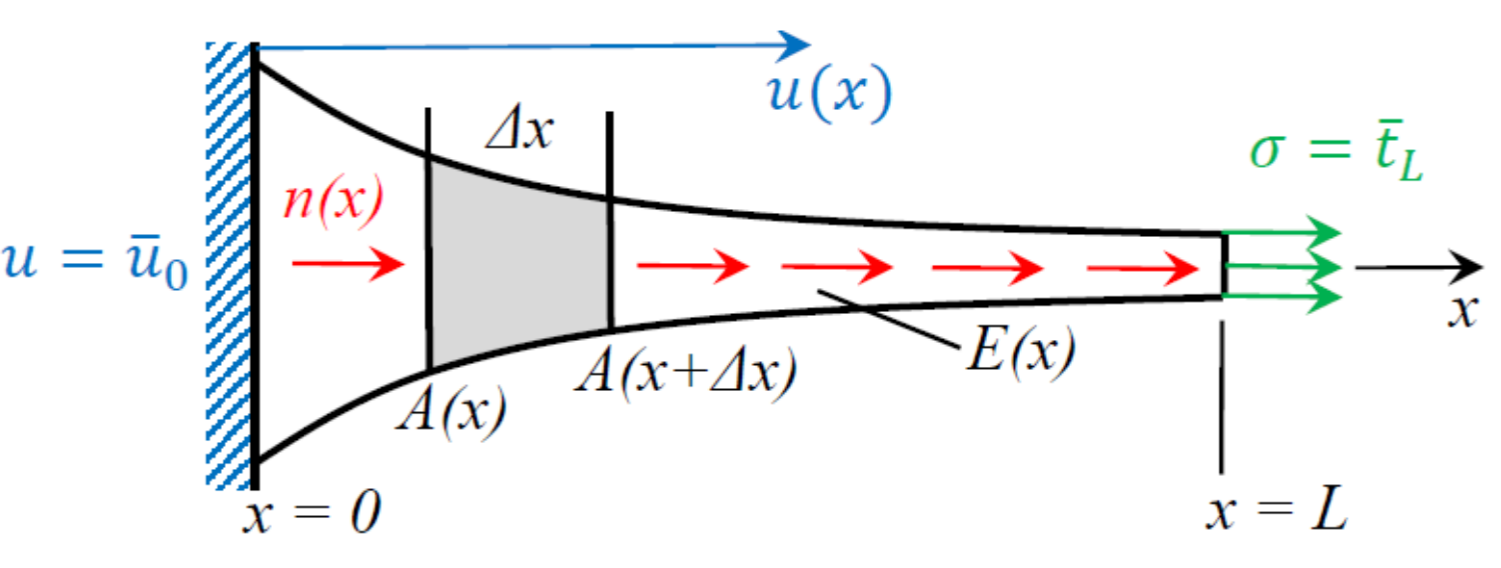
\includegraphics[height=2.3cm,keepaspectratio]{../Grafiken/V7_Stab_skizze.png}
  \end{center}
  \vspace{-1.2em}
  \begin{columns}[T,onlytextwidth]
    % ---- Starke Form ----
    \begin{column}{0.41\textwidth}
      \textbf{Starke Form}\\[0.2em]
      \begin{tcolorbox}[colback=orange!10, colframe=blue!70!black,
          boxrule=1.5pt, left=4pt, right=4pt, top=2pt, bottom=2pt]
        \small
        \begin{tabular}{@{}l@{\;}l@{}}
          (a) & $\dfrac{d}{dx}\!\left(AE\dfrac{du}{dx}\right)+n=0$,\; $x\in(0,L)$\\[0.8em]
          (b) & $u(0)=\bar{u}_0$\\[0.3em]
          (c) & $\sigma(L)=Eu'(L)=\bar{t}_L$
        \end{tabular}
      \end{tcolorbox}
      \vspace{0.2em}
      \begin{itemize}\footnotesize
        \item[(a)] muss punktweise erfüllt sein $\rightarrow$ $x\in(0,L)$
        \item[(c)] ist die kinetische Randbed.\ $\rightarrow$ $\sigma(L)=\bar{t}_L$
        \item[(a)] beinhaltet zweifache Ableitungen von $u$
      \end{itemize}
    \end{column}
    % ---- Doppelpfeil ----
    \begin{column}{0.05\textwidth}
      \centering\vspace{1.8em}
      {\large$\Longleftrightarrow$}
    \end{column}
    % ---- Schwache Form ----
    \begin{column}{0.54\textwidth}
      \textbf{Schwache Form}\\[0.2em]
      \begin{tcolorbox}[colback=orange!10, colframe=orange!80!black,
          boxrule=1.5pt, left=4pt, right=4pt, top=2pt, bottom=2pt]
        \small
        \begin{tabular}{@{}l@{\;}l@{}}
          (a) & $\displaystyle\int_0^L AE\,\hlg{\dfrac{dg}{dx}}\hlg{\dfrac{du}{dx}}\dd x
                = \bar{t}_L(gA)\big|_L + \int_0^L \hlg{g}n\,\dd x \quad \forall \hlg{g}$\\[0.8em]
          (b) & $u(0)=\bar{u}$\\[0.3em]
          (c) & $g(0)=0\quad\forall g$
        \end{tabular}
      \end{tcolorbox}
      \vspace{0.2em}
      \begin{itemize}\footnotesize
        \item[(a)] ist eine variationale Gl.\ $\rightarrow$ $\forall g$ mit $g(0)=0$
        \item[(a)] beinhaltet die kinetische Randbed.\ $\rightarrow$ $\bar{t}_L(gA)|_L$
        \item[(a)] enthält nur erste Ableitungen von $u$ $\rightarrow$ $\dfrac{du}{dx}$
        \item[(a)] ist in Integralform
           
      \end{itemize}
    \end{column}
  \end{columns}
\end{frame}

% ---------------------------------------------------------------------------
% Nebenbemerkung: Prinzip der virtuellen Arbeit
% ---------------------------------------------------------------------------
\begin{frame}{Nebenbemerkung: Interpretation Prinzip der virtuellen Arbeit}

  \small
  Die Gewichtsfunktion $g(x)$ wird als \textbf{virtuelle Verschiebung} $\delta u(x)$ interpretiert
  (mit $g(0)=0$, d.\,h.\ die virtuelle Verschiebung verschwindet an kinematischen RB).

  \vspace{1.0em}
  \begin{center}
  \[
    \underbrace{%
      \int_0^L AE\,\frac{dg}{dx}\frac{du}{dx}\dd x
    }_{\delta W^{\mathrm{int}}:\;\text{innere virtuelle Arbeit}}
    \;=\;
    \underbrace{%
      \bar{t}_L\,(gA)\big|_L
    }_{\substack{\text{virtuelle Arbeit}\\\text{der Randlast}}}
    \;+\;
    \underbrace{%
      \int_0^L g\,n\,\dd x
    }_{\substack{\text{virtuelle Arbeit}\\\text{der Streckenlast}}}
    \;=:\;
    \delta W^{\mathrm{ext}}
    \qquad\forall g
  \]
  \end{center}

  \vspace{0.5em}
  \begin{center}
  \[
    \Longleftrightarrow\quad
    \underbrace{\delta W^{\mathrm{ext}} - \delta W^{\mathrm{int}}}_{=\;\delta W^{\mathrm{tot}}}
    = 0 \qquad \forall g
  \]
  \end{center}

  \vspace{0.5em}
  \begin{itemize}
    \item $\delta W^{\mathrm{int}}$: Formänderungsenergie durch virtuelle Verzerrungen $\dfrac{dg}{dx}$
    \item $\delta W^{\mathrm{ext}}$: Arbeit der äußeren Kräfte (Randlast + Streckenlast) entlang $g$
    \item Gleichgewicht $\Leftrightarrow$ die gesamte virtuelle Arbeit verschwindet für alle $g$
  \end{itemize}

\end{frame}




% ---------------------------------------------------------------------------
% Nebenbemerkung: Terminologie Randbedingungen
% ---------------------------------------------------------------------------
\begin{frame}{Nebenbemerkung: Terminologie Randbedingungen}
  \begin{columns}[T,onlytextwidth]
    \begin{column}{0.48\textwidth}
      \centering
      \begin{tcolorbox}[colback=orange!10, colframe=blue!70!black,
          boxrule=1.5pt, left=6pt, right=6pt, top=5pt, bottom=5pt,
          title={\textbf{Verschiebungs-RB}}, fonttitle=\small\bfseries]
        \small\centering
        \textbf{kinematische RB}\\[0.3em]
        = \textbf{wesentliche RB} = \textbf{geometrische RB}\\[0.3em]
        = \textbf{Dirichlet-RB}\\[0.6em]
        z.\,B.\; $u(0) = \bar{u}_0$\\[0.3em]
        \footnotesize(vorgeschriebene Verschiebung)
      \end{tcolorbox}
    \end{column}
    \begin{column}{0.48\textwidth}
      \centering
      \begin{tcolorbox}[colback=orange!10, colframe=orange!80!black,
          boxrule=1.5pt, left=6pt, right=6pt, top=5pt, bottom=5pt,
          title={\textbf{Spannungs-RB}}, fonttitle=\small\bfseries]
        \small\centering
        \textbf{kinetische RB}\\[0.3em]
        = \textbf{natürliche RB} = \textbf{dynamische RB}\\[0.3em]
        = \textbf{Neumann-RB}\\[0.6em]
        z.\,B.\; $\sigma(L) = \bar{t}_L$\\[0.3em]
        \footnotesize(vorgeschriebene Kraft/Spannung)
      \end{tcolorbox}
    \end{column}
  \end{columns}

  \vspace{1.0em}
  \small
  \begin{itemize}
    \item Kinematische/Dirichlet-RB müssen von der Ansatzfunktion \textbf{explizit erfüllt} werden.
    \item Kinetische/natürliche/Neumann-RB gehen \textbf{automatisch} über den Randterm in die schwache Form ein.
  \end{itemize}
\end{frame}

\end{document}
